\chapter{Road Network Properties}
\label{ch:properties}

This chapter provides an empirical analysis of several fundamental properties of real-world road networks.
We investigate key characteristics such as separator sizes, degree distribution, planarity, hierarchy, and diameter to establish a baseline understanding of these networks.
These empirical findings serve as a foundation for the synthetic graph generation and analysis presented in subsequent chapters.

\section{Separator Sizes}
\label{sec:empirical_analysis}

To empirically investigate the relationship between graph size and separator size in road networks, we analyze the DIMACS Europe dataset provided by PTV \cite{ptv_group_dimacs-europe_2009}.
We take the largest connected component of this graph and make it undirected by ignoring edge directions as we are primarily interested in the topological structure rather than the specific flow direction of traffic.
A crucial first step in our research is to empirically validate the scaling of these separators.
We seek to determine if they scale near \(\bigO{n^{1/3}}\), as suggested by prior work \cite{dibbelt_customizable_2016}, or if an alternative scaling, like \(\bigO{n^{1/2}}\), merely appears smaller due to a low constant factor.
\cref{fig:separator_size_vs_graph_size} plots the size of separators against the size of the corresponding subgraphs from which they are computed.
Each data point \( (x, y) \) in this figure signifies that a subgraph containing \( x \) nodes possesses a separator of size \( y \).
The data points are generated by recursively applying nested dissection, computing separators first for the original graph and then for the subgraphs induced at each subsequent level.

\begin{figure}[tbhp]
    \centering
    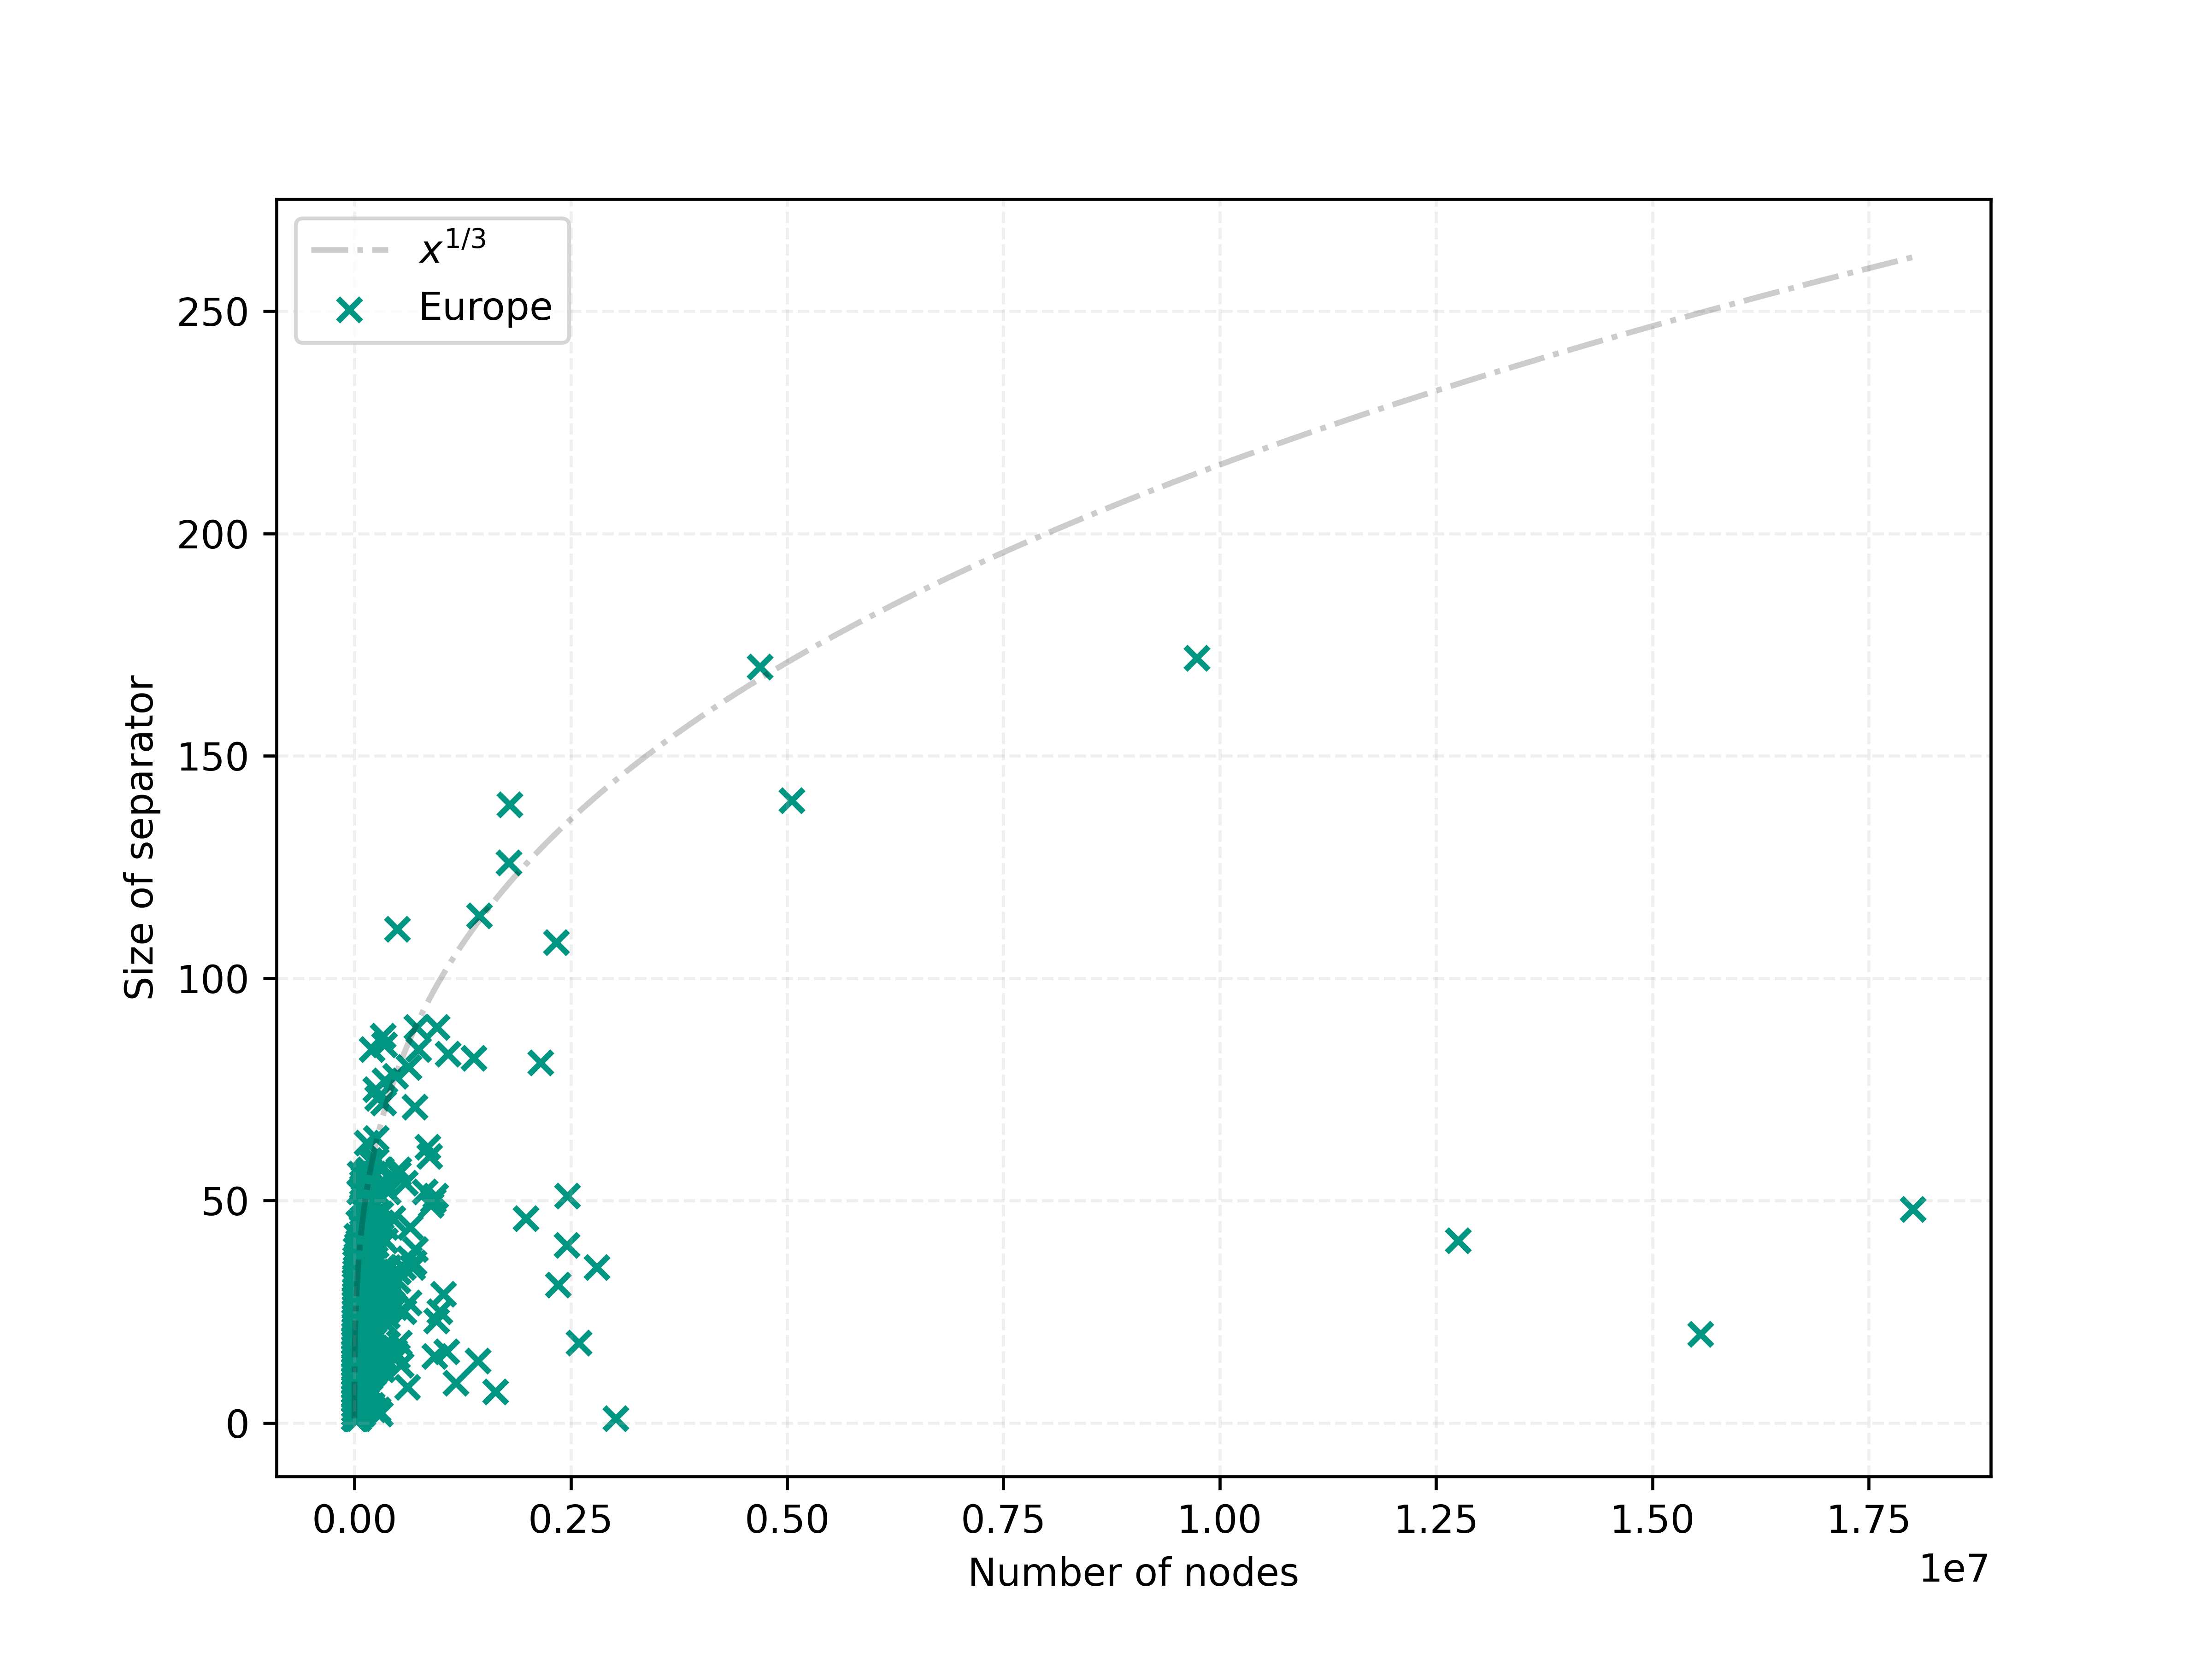
\includegraphics[width=0.7\linewidth]{graphics/Europe.png}
    \caption{Empirical separator size versus subgraph size for the Europe road network. Each point represents a subgraph and its corresponding separator size. Separators were computed using InertialFlowCutter.}
    \label{fig:separator_size_vs_graph_size}
\end{figure}

Initial observations reveal outliers, particularly for very large subgraphs corresponding to continental or country scales.
Specifically, analysis of the top-level separator structure for the Europe graph shows that the Scandinavian peninsula can be disconnected via separators significantly smaller than the general trend would suggest.
This is due to specific geographic bottlenecks, as illustrated in \cref{fig:europe_top_separator}.
Such outliers at the largest scales appear to be heavily influenced by macroscopic geographic features rather than intrinsic network structure representative of typical road networks.
Consequently, these data points may not accurately reflect the general separator properties inherent in the finer structure of the road network graph.
To mitigate the influence of these large-scale geographical artifacts and focus on more representative structural properties, our analysis primarily considers subgraphs with fewer than 10,000,000 nodes.

\begin{figure}[tbhp]
    \centering
    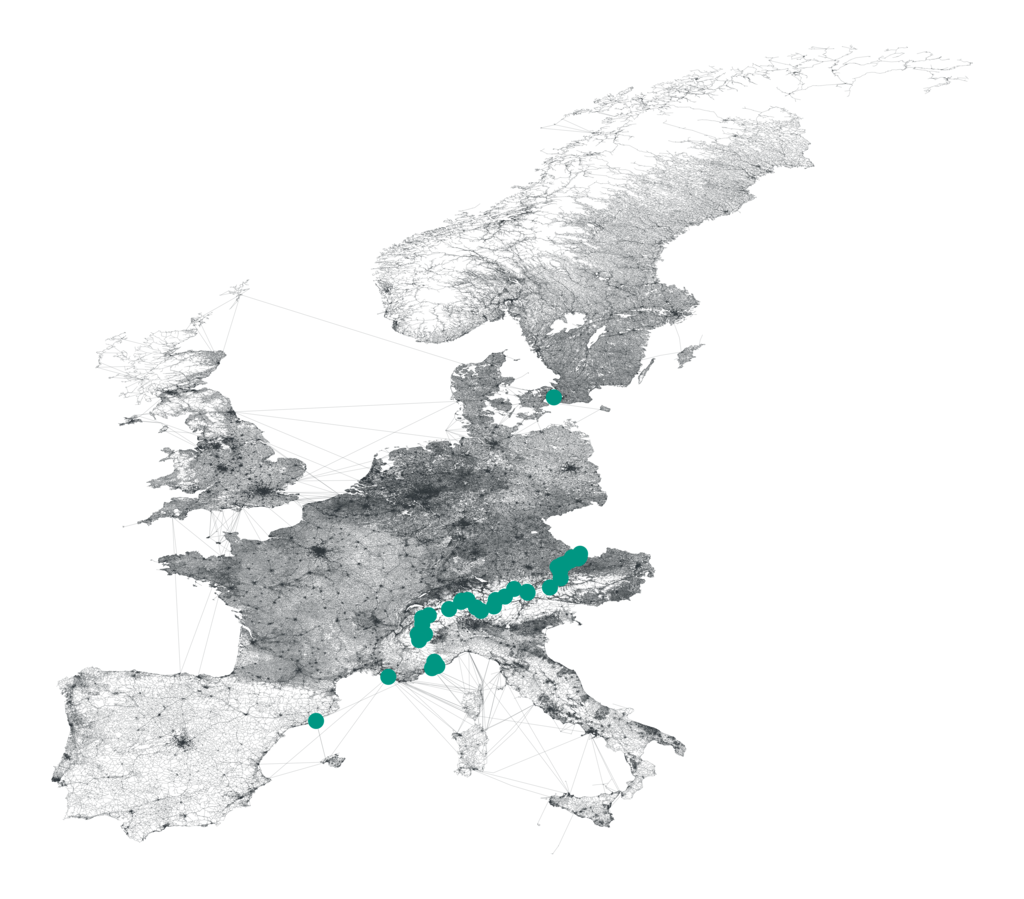
\includegraphics[width=0.6\linewidth]{graphics/europe-top-level-sep.png}
    \caption{Illustration of a geographically influenced outlier at the continental scale: removal of a few nodes disconnects the entire Scandinavian peninsula.}
    \label{fig:europe_top_separator}
\end{figure}

For enhanced visibility, particularly concerning the numerous data points corresponding to smaller subgraphs, and to avoid overrepresentation of larger subgraphs, we will also present data on a log-log scale.
This logarithmic scaling offers the additional advantage that a polynomial relationship between separator size \( y \) and subgraph size \( x \), such as \( y \propto x^c \), manifests as a linear trend in the log-log plot, facilitating the identification of potential power-law dependencies.
Furthermore, to improve the interpretability of the visualization and emphasize the underlying trend over individual fluctuations or outliers present at various scales, the data points are aggregated into bins.
Let \( b \) be the number of bins chosen for the aggregation.
Let \( x_{\max} \) denote the maximum observed subgraph size, assuming \( x_{\max} > 0 \).
A data point \( (x, y) \) is assigned to the bin with index \( \floor{\frac{x \cdot b}{x_{\max}}} \).
After assigning all points to their respective bins, a single representative point is computed for each non-empty bin.
This representative point \( (\overline{x}_i, \overline{y}_i) \) for bin \( i \) is determined by calculating the arithmetic mean of the \( x \) coordinates and the arithmetic mean of the \( y \) coordinates of all data points \( (x, y) \) assigned to bin \( i \).
A primary consideration for using the arithmetic mean was the nature of subsequent analysis steps, such as curve fitting.
While methods like box plots offer detailed distributional insights, they do not provide the single-point representation required for these analyses.
Furthermore, the choice of the mean over the median, which is known for its robustness to outliers, was deliberate in this context.
Outliers within bins are not necessarily disregarded as noise but are considered potentially informative data points reflecting relevant variations.
Supporting this decision are the mean's straightforward calculation, computational efficiency, and clear interpretation as the centroid or center of mass of the points within the bin.

When constructing the log-log plot, this binning procedure is applied to the logarithmically transformed data.
\cref{fig:separator_size_loglog} illustrates the binned data points on logarithmic axes alongside the non-binned data.

\begin{figure}[tbhp]
    \begin{subfigure}{0.49\linewidth}
        \centering
        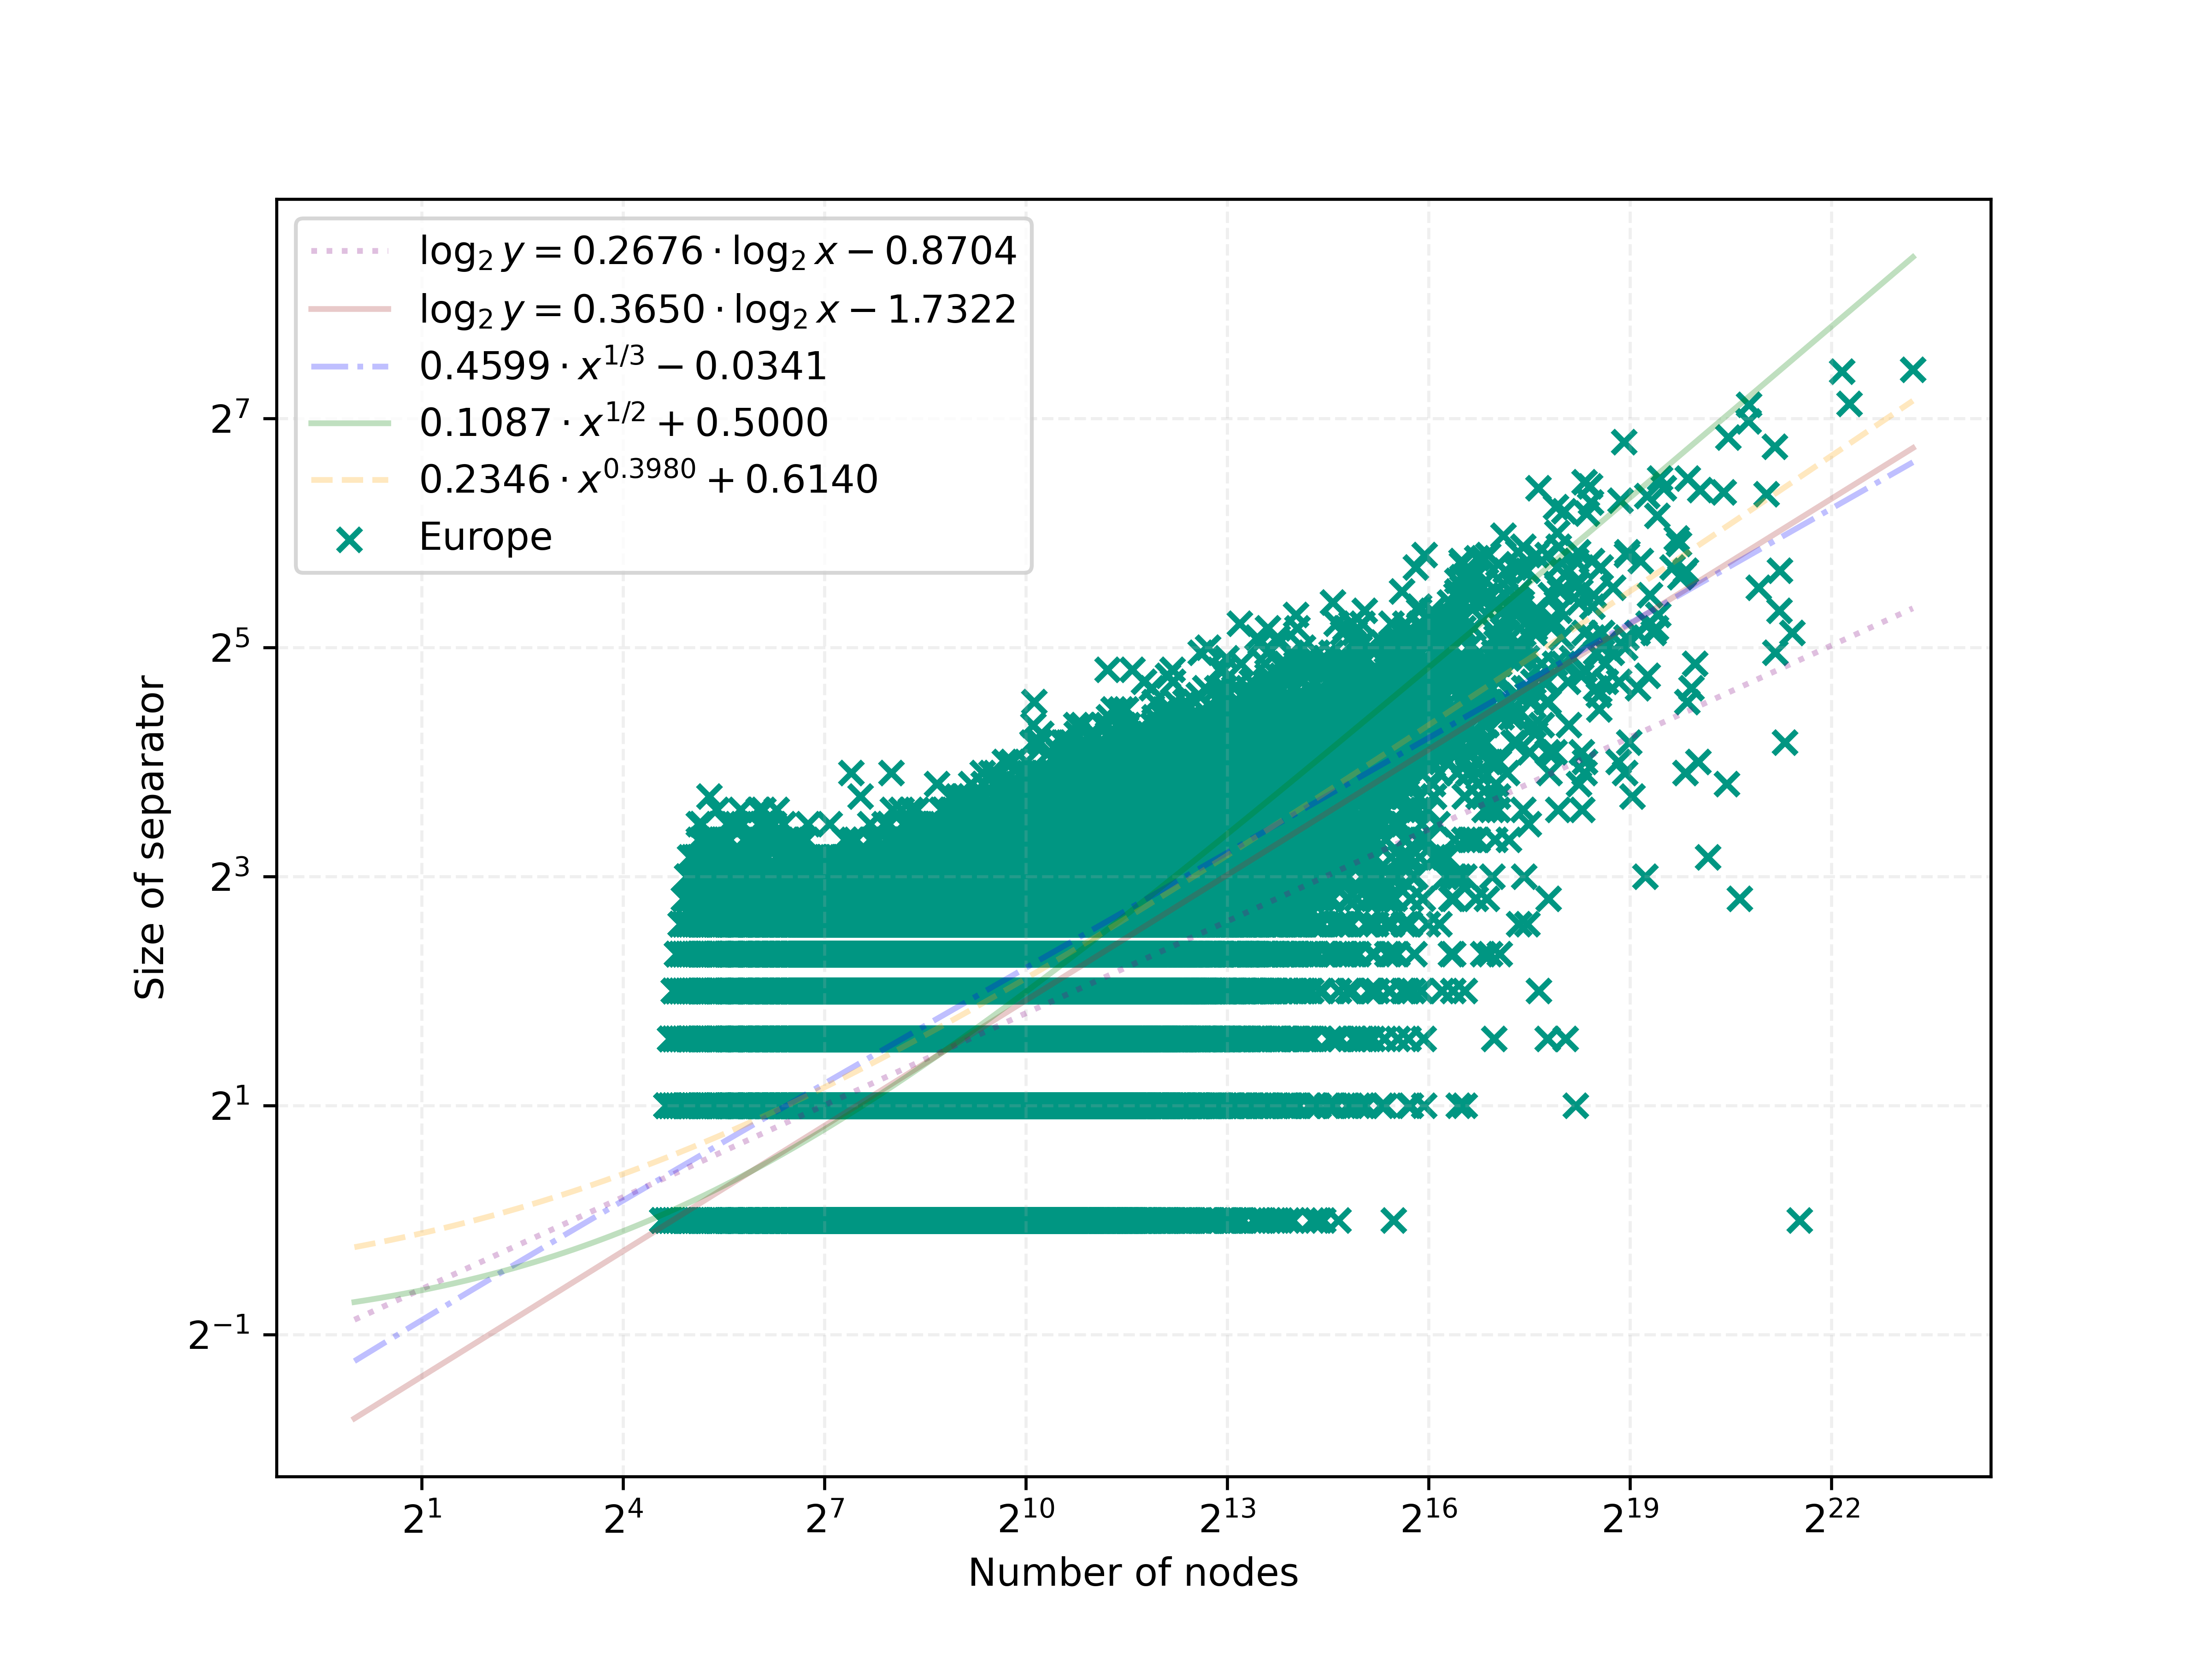
\includegraphics[width=\linewidth]{graphics/Europe_non_binned.png}
        \caption{Non-binned separator sizes.}
        \label{fig:separator_size_loglog_non_binned}
    \end{subfigure}
    \hfill
    \begin{subfigure}{0.49\linewidth}
        \centering
        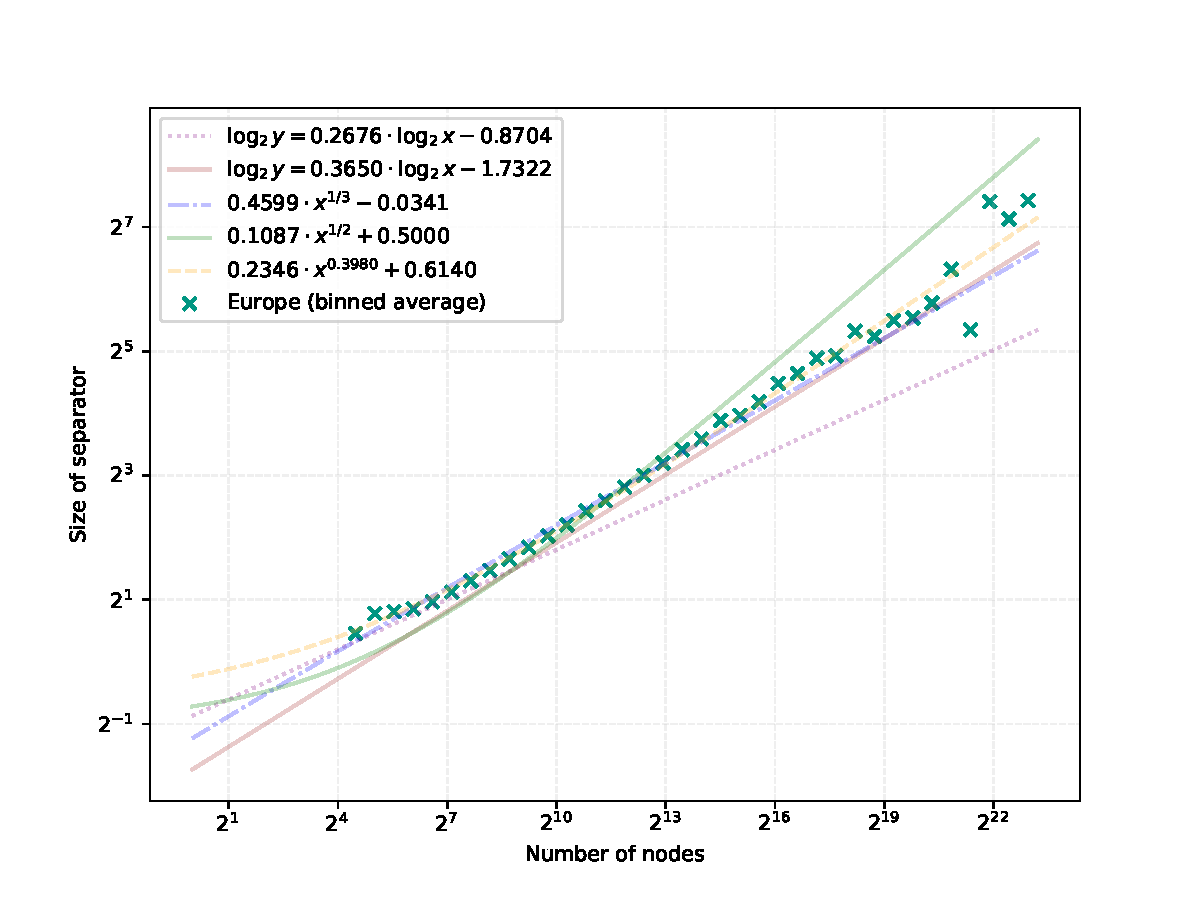
\includegraphics[width=\linewidth]{graphics/Europe-binned.pdf}
        \caption{Binned average separator sizes.}
        \label{fig:separator_size_loglog_binned}
    \end{subfigure}
    \caption{Separator sizes of Europe on logarithmic axes (subgraphs < 10M nodes). Separators were computed using InertialFlowCutter (tests with FlowCutter and KaHIP yielded similar asymptotic scaling).}
    \label{fig:separator_size_loglog}
\end{figure}

To quantify the relationship between separator size \( y \) and subgraph size \( x \), we perform statistical curve fitting on the empirical data.
A preliminary linear regression applied to the logarithmically transformed data across all points yields a fitted line \( \log y \approx 0.2676 \log x - 0.8704 \).
This initial fit suggests a scaling behavior close to \( \bigO{x^{0.2676}} \), seemingly better than the hypothesized \( \bigO{x^{1/3}} \).
However, this result is likely skewed by the large number of small subgraphs, which may not fully represent the scaling trend at larger sizes.
To test this hypothesis, we perform a second regression exclusively on data points corresponding to subgraphs with more than \( 2^8 = 256 \) vertices.
This analysis yields the relationship \( \log y \approx 0.3650 \log x - 1.7322 \).

We report these coefficients to four decimal places in accordance with scientific reporting conventions.
However, we acknowledge that this level of precision might overstate the certainty of the fit, given the inherent noise in empirical measurements from complex graph algorithms.
Minor variations in experimental conditions, such as changing the random seed used in the nested dissection algorithm, can cause slight fluctuations in these fitted parameters.
Therefore, the reported values should be interpreted as indicative of the general trend rather than as exact constants.

We also explore direct non-linear curve fitting to the original data points using several functional forms.
Fitting \( y = a \cdot x^{1/3} + b \) results in \( y \approx 0.4599 \cdot x^{1/3} - 0.0341 \) with an \( R^2 \) value of \( 0.4724 \).
Fitting \( y = a \cdot x^{1/2} + b \) yields \( y \approx 0.1087 \cdot x^{1/2} + 0.5000 \), but with a very low \( R^2 \) value of \( 0.0873 \), suggesting that a square-root dependency is unlikely.
A more general power-law fit \( y = a \cdot x^c + b \) results in \( y \approx 0.2346 \cdot x^{0.3980} + 0.6140 \) with an \( R^2 \) value of \( 0.4832 \).
While these direct fits indicate a scaling exponent potentially closer to \( 0.4 \) than to \( 1/3 \) or \( 1/2 \), the overall \( R^2 \) scores remain relatively low, indicating only a moderate goodness of fit.
These fitted curves are visualized in \cref{fig:separator_size_loglog}.
The fitted lines from the non-binned data (\cref{fig:separator_size_loglog_non_binned}) are reproduced in \cref{fig:separator_size_loglog_binned} to facilitate comparison with the binned averages; visual alignment may differ due to the binning process.

Observations from the binned log-log plot in \cref{fig:separator_size_loglog_binned} suggest that the linear relationship between \( \log y \) and \( \log x \) is most consistent within a specific range of subgraph sizes.
The data appear particularly stable for subgraph sizes \( x \) between approximately \( 2^7 \) and \( 2^{18} \) nodes.
For subgraphs smaller than \( 2^7 \) nodes, a slight upward deviation is discernible, potentially reflecting behavior closer to grid-like structures at very small scales.
For subgraphs larger than \( 2^{18} \) nodes, the increased scatter might be attributed to the limited number of data points available for aggregation in these higher size ranges.

To obtain a more robust estimate of the scaling exponent, we focus our analysis on the data within this more stable range (\( 2^7 \le x \le 2^{18} \)).
Furthermore, performing the linear regression on the binned data points offers two key advantages.
Firstly, binning averages out the influence of individual outliers within each bin.
Secondly, it gives more equal weight to different orders of magnitude in subgraph size, mitigating the numerical dominance of the numerous small subgraphs in the dataset.

Applying linear regression to the mean coordinates of the bins within the selected range on the log-log scale yields the fitted line:
\[ \log y \approx 0.3702 \log x - 1.5512\ \quad\iff\quad y \approx 0.3411 \cdot x^{0.3702}\]
This fit demonstrates an exceptionally high coefficient of determination (\( R^2 \approx 0.9994 \)), indicating that the linear model explains almost all the variance in the binned log-transformed data.
The statistical significance of the slope is confirmed by an extremely low p-value (\( p \approx 1.64 \times 10^{-20} \)).

\begin{figure}[tbhp]
    \centering
    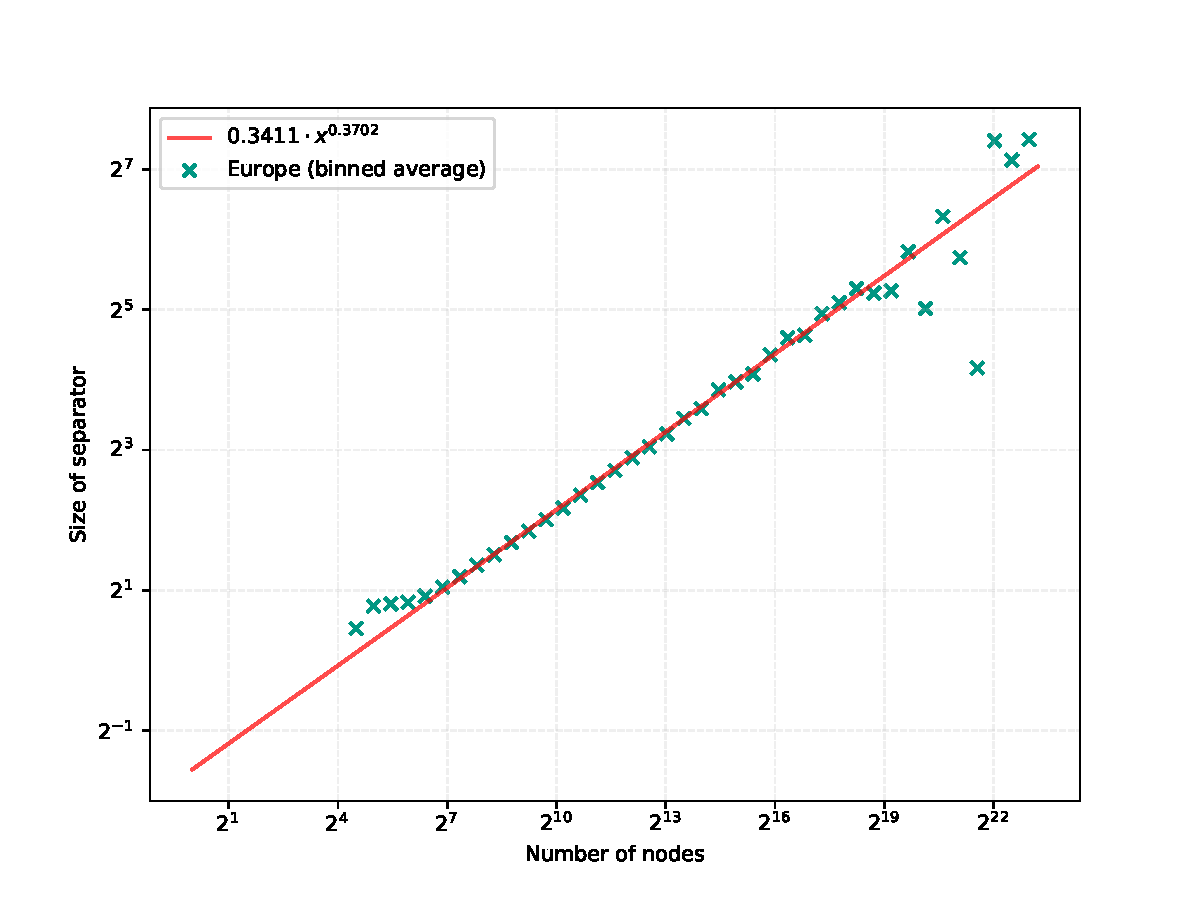
\includegraphics[width=0.7\linewidth]{graphics/EuropeShowFit.pdf}
    \caption{Linear regression fit to the binned data of separator size versus subgraph size, plotted on logarithmic axes. The regression considers only bins corresponding to subgraph sizes (\(x\)) in the range \( 2^7 \le x \le 2^{18} \). Separators were computed using InertialFlowCutter (tests with FlowCutter and KaHIP yielded similar asymptotic scaling).}
    \label{fig:separator_size_loglog_fit}
\end{figure}

Visually, this line provides an excellent fit to the binned data points within the considered range, as illustrated in \cref{fig:separator_size_loglog_fit}.
The slope of \( 0.3702 \) in the log-log regression corresponds to the exponent in the power-law relationship \( y \propto x^c \).
Based on the high quality of the fit (\( R^2 \approx 0.9994 \)) and the statistical significance of the result, we can state with high confidence that the observed scaling behavior is close to, yet slightly above, \( \bigO{n^{1/3}} \).

\paragraph{Initial Deviations in Separator Scaling}
Empirical studies of road networks reveal a notable deviation in separator scaling for small subgraphs.
This deviation is particularly apparent for subgraphs containing approximately \(2^6\) vertices, where separator sizes are often larger than the general scaling trend would suggest, as can be observed in \cref{fig:separator_size_loglog_non_binned}.
\cref{fig:real_europe_hist} presents a histogram that further visualizes the distribution of these separator sizes.
This phenomenon corresponds with the observation of a higher meshedness coefficient for smaller, denser urban cores, as discussed in \cref{sec:degree_distribution}.
The more grid-like, densely connected structure implied by a higher meshedness may contribute to these comparatively larger separators at smaller scales.

\begin{figure}[tbhp]
    \centering
    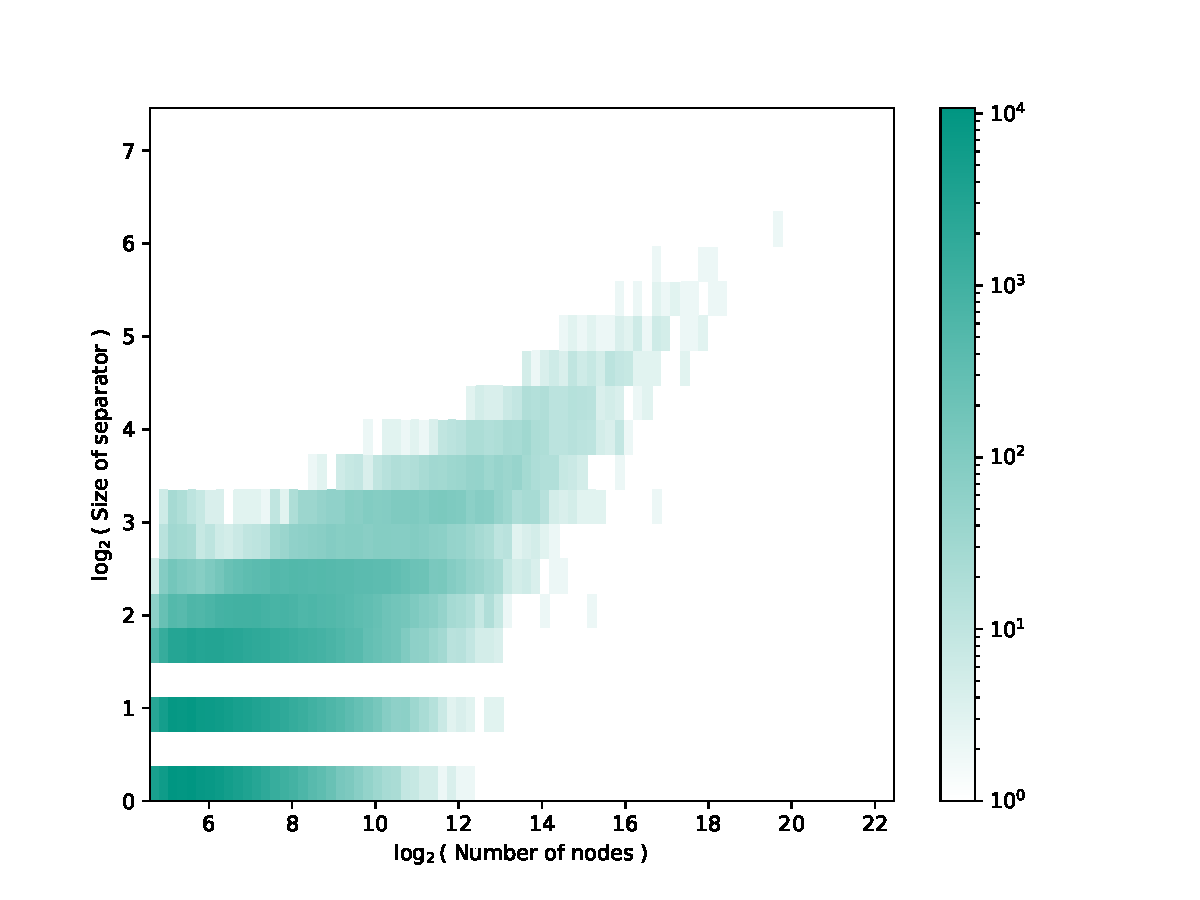
\includegraphics[width=0.7\linewidth]{graphics/Germany-hist.pdf}
    \caption{Histogram illustrating the distribution of separator sizes for road networks. A slight increase in relative separator size is observed for graphs with approximately \(2^6\) nodes. Separators were computed using InertialFlowCutter (tests with FlowCutter and KaHIP yielded similar asymptotic scaling).}
    \label{fig:real_europe_hist}
\end{figure}

\section{Degree Distribution}
\label{sec:degree_distribution}

Road networks are characteristically sparse graphs.
The DIMACS Europe road network dataset from PTV \cite{ptv_group_dimacs-europe_2009}, used in our experiments, exemplifies this with an average vertex degree of approximately \(2.5\).
\cref{fig:degree_dist_europe} presents this network's degree distribution, which reveals that a vast majority of vertices (approximately \(99.8\%\)) have a degree less than 5.
The maximum degree observed in this dataset is 12, attained by a single node.

\begin{figure}[tbhp]
    \centering
    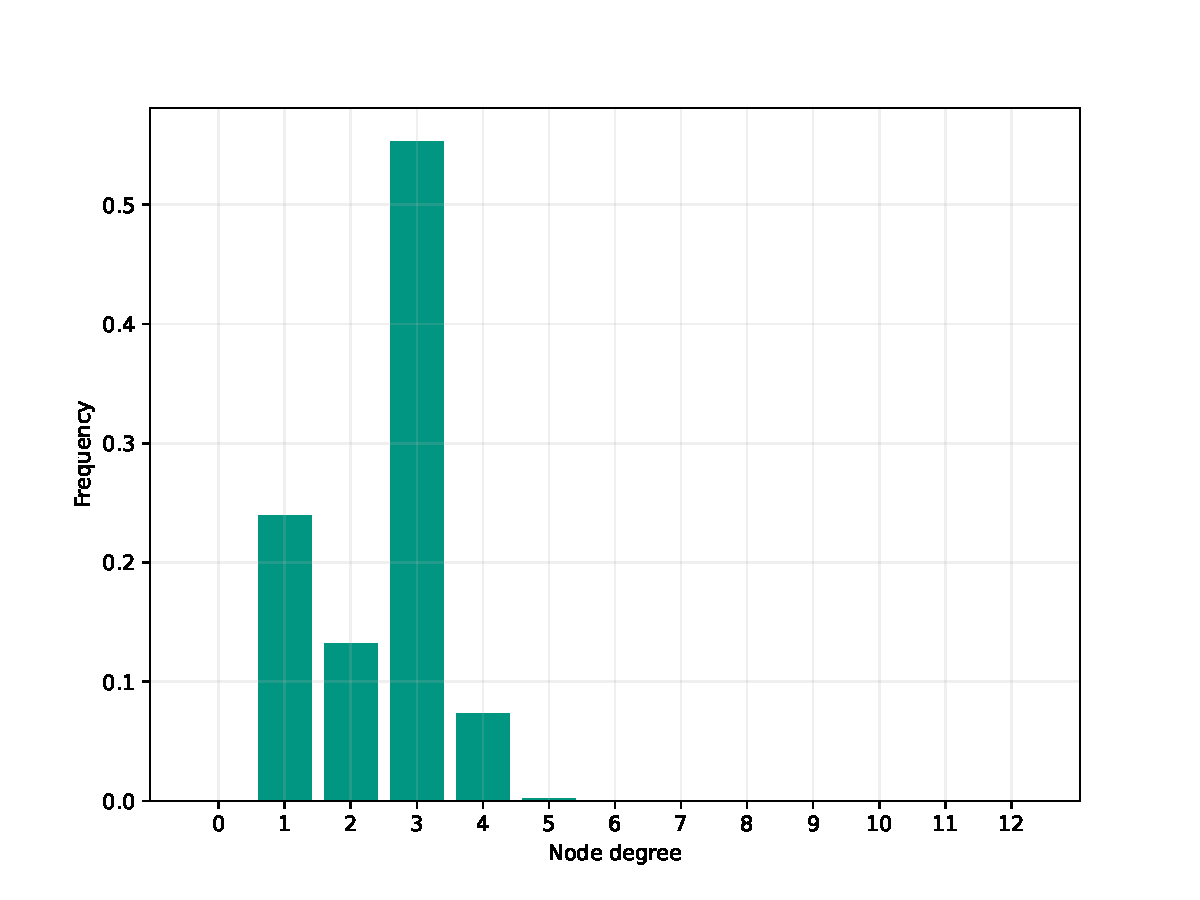
\includegraphics[width=0.6\linewidth]{graphics/degree_overview_europe.pdf}
    \caption{Degree distribution of the DIMACS Europe road network \cite{ptv_group_dimacs-europe_2009}. The x-axis represents vertex degree, and the y-axis indicates the fraction of vertices.}
    \label{fig:degree_dist_europe}
\end{figure}

\paragraph{Implications for Other Structural Metrics}
\label{sec:degree_related_metrics}

The degree distribution and overall sparsity also influence other structural metrics, particularly when considering the near-planar nature of road networks.
One such metric for planar-like graphs is the meshedness coefficient, \(\alpha\), which quantifies the density of cycles or bounded faces within a planar graph \cite{buhl_topological_2006}.
It is calculated as the ratio of a graph's actual number of bounded faces (\(m - n + 1\)) to the maximum possible for a planar graph with \(n\) vertices and \(m\) edges, via the formula \(\alpha = \frac{m - n + 1}{2n - 5}\).
This coefficient ranges from 0 for trees to 1 for maximal planar graphs.
Buhl et al. suggest that this coefficient can also be used to gauge a network's robustness to disconnections and its cost in terms of total edge length \cite{buhl_topological_2006}.
For the DIMACS Europe road network, after applying a planarization procedure (detailed in \cref{sec:approach:planarity}), we compute a meshedness coefficient \(\alpha \approx 0.1166\).
This relatively low value underscores the network's general sparsity and somewhat tree-like macroscopic structure.
For context, the meshedness coefficient for a square grid approaches \(0.5\) as \(n \to \infty\), while a full Delaunay triangulation, as an almost maximal planar graph, approaches 1.
In contrast to the continental scale, urban cores are typically more densely meshed.
To illustrate this, we analyze the inner-city structure of Karlsruhe, a sub-region available within the PTV/DIMACS dataset.
Representations of roads often include long chains of degree-2 vertices that model segments rather than structurally significant junctions.
Such modeling can artificially skew the meshedness coefficient to lower values because adding these degree-2 vertices increases \(n\) without increasing the graph's cycle count.
Therefore, to analyze the underlying junction-based topology independent of this modeling artifact, contracting degree-2 vertices is a valuable normalization step.
After applying this contraction, the graph for Karlsruhe's inner city yields a meshedness coefficient of approximately \(0.25\).
This higher value reflects the more grid-like layout characteristic of dense urban centers.
Applying this same normalization step to the entire DIMACS Europe graph has a less pronounced impact, increasing its meshedness coefficient only slightly from \(0.1166\) to \(0.1317\).

\section{Planarity}
\label{sec:approach:planarity}

Road networks can be modeled as nearly planar graphs, meaning they permit an embedding in the plane with a limited number of edge crossings.
Empirical evidence suggests that the number of such crossings in real-world road networks is typically on the order of \(\bigO{n}\), a sub-linear count relative to the number of edges \cite{eppstein_studying_2008}.
It is a well-known result in graph theory that planar graphs admit \(\frac{2}{3}\)-balanced separators of size \(\bigO{n^{1/2}}\) \cite{lipton_separator_1979}.
A relevant inquiry is whether the near-planarity of road networks is a critical feature that influences their separator properties, or if the occasional non-planar elements are merely incidental.
This prompts the question of how separator sizes are affected when road networks are transformed into strictly planar graphs.

To obtain a planar representation, we begin with the existing graph structure where vertices possess associated geometric coordinates.
Each edge is interpreted as the straight line segment connecting the coordinates of its incident vertices.
The algorithm then identifies all geometric intersection points between these line segments.
A new vertex is introduced into the graph at the coordinates of each detected intersection, provided this point does not coincide with an existing vertex.
Any original edge containing one or more such intersection points is then removed and replaced by a sequence of new, shorter edges that connect the original endpoints and the new intersection vertices in their linear order.
This process transforms the initial graph into a planar graph embedding by explicitly representing all edge crossings as vertices.
For efficient execution, we utilize a spatial index over the bounding boxes of all edges.
This structure enables rapid identification of potential intersections by querying for overlapping bounding boxes, which can then be verified for actual crossings.
While other approaches exist, such as the Bentley-Ottmann algorithm for general line segment intersection \cite{bentley_algorithms_1979} or linear-time algorithms tailored for graphs with a sublinear number of crossings \cite{eppstein_linear-time_2010}, our spatial index-based method is chosen for its implementation simplicity, as performance is not a critical concern for this pre-processing step.
Since a single edge may cross multiple other edges, intersection points are sorted along each original edge before new sub-edges are introduced.
Pseudo-code for this planarization algorithm is provided in \cref{alg:planarization}.

\begin{algorithm}[tbhp]
    \Input{Non-planar graph \(G=(V, E, pos)\).}
    \Output{Planarized version of G.}
    \BlankLine
    spatial\_index \(\longleftarrow\) load(bounding\_boxes(E))\;
    crossings \(\longleftarrow\) \{\}\;
    \ForAll{e in E}{
        \ForAll{candidates c in spatial\_index.query(e)}{
            \If{c intersects e} {
                crossings[e].append(c)\;
                crossings[c].append(e)\;
            }
        }
    }
    \ForAll{(e, crossed) in crossings}{
        G.remove(e)\;
        vertices \(\longleftarrow\) get\_intersection\_vertices(e, crossed)\;
        sort\_vertices\_along\_edge(e, vertices)\;
        add\_new\_edges(e, vertices)\;
    }
    \caption{Simple planarization algorithm \label{alg:planarization}}
\end{algorithm}

We apply this planarization method to several real-world road networks.
The Karlsruhe network, with approximately 120,000 nodes, has around 2,500 crossings.
The Germany network, comprising about 6 million nodes, has approximately 100,000 crossings.
Finally, the Europe network, with around 18 million nodes, contains about 300,000 crossings.
These numbers are a little higher than intersection counts on the order of \(n^{1/2}\) reported in some prior studies, but are of a comparable order of magnitude \cite{eppstein_studying_2008}.
The differences could be explained by our modeling of edges as straight lines rather than more complex curves, and might be mitigated by using a more detailed road network model like OpenStreetMap.

Analysis of separator sizes shows minimal variation post-planarization.
We identify \(\frac{2}{3}\)-balanced separators with sizes still scaling approximately as \bigO{n^{1/3}}, aligning with the values from the original non-planar graphs.
A comparison of the separator sizes in the planar and non-planar versions of the Europe network is depicted in \cref{fig:germany_planar_vs_non_planar}.

\begin{figure}[tbhp]
    \centering
    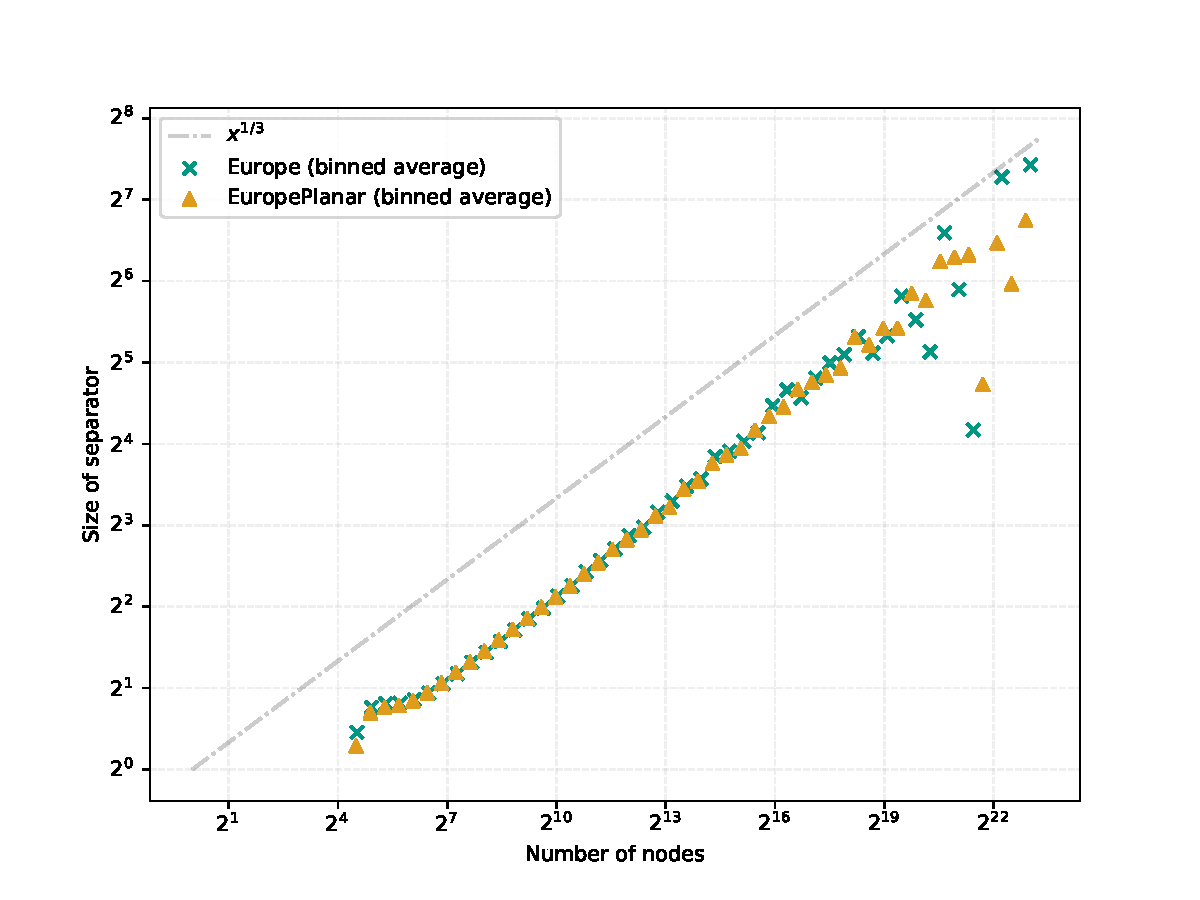
\includegraphics[width=0.6\linewidth]{graphics/EuropePlanarVsNonPlanar.pdf}
    \caption{Comparison of separator sizes in the European road network: planar vs. non-planar versions. Separators were computed using InertialFlowCutter (tests with FlowCutter and KaHIP yielded similar asymptotic scaling).}
    \label{fig:germany_planar_vs_non_planar}
\end{figure}

Our findings indicate that separators in non-planar road networks closely resemble those in their planarized counterparts in terms of overall scaling.
However, a separator from the original graph is not always directly valid in the planarized version, as edge crossings can create new paths between previously separated components.
We investigated this by traversing a single arm of a nested dissection and checking if the separators for the original subgraphs remain valid in their planarized versions.
Approximately one-third of these separators can be applied directly without modification, this is more probable for smaller subgraphs that are less likely to contain edge crossings.
When a separator is invalidated by the new topology, different outcomes are possible.
In many cases, an original separator must be augmented with additional nodes to restore the partition, resulting in a slightly larger separator.
\cref{fig:karlsruhe_planar_vs_non_planar} provides a real-world example, visualizing how a separator from the non-planar Karlsruhe network has to be augmented to remain valid after planarization.

The new structure created by planarization can also reveal a new, more efficient separator that is smaller than the original, as shown in the example in \cref{fig:planarization_reduces_separator}.
Conversely, there are also rare cases in which no better separator can be found in the planarized graph, as illustrated in \cref{fig:planarization_increases_separator}.

\begin{figure}[tbhp]
    \centering
    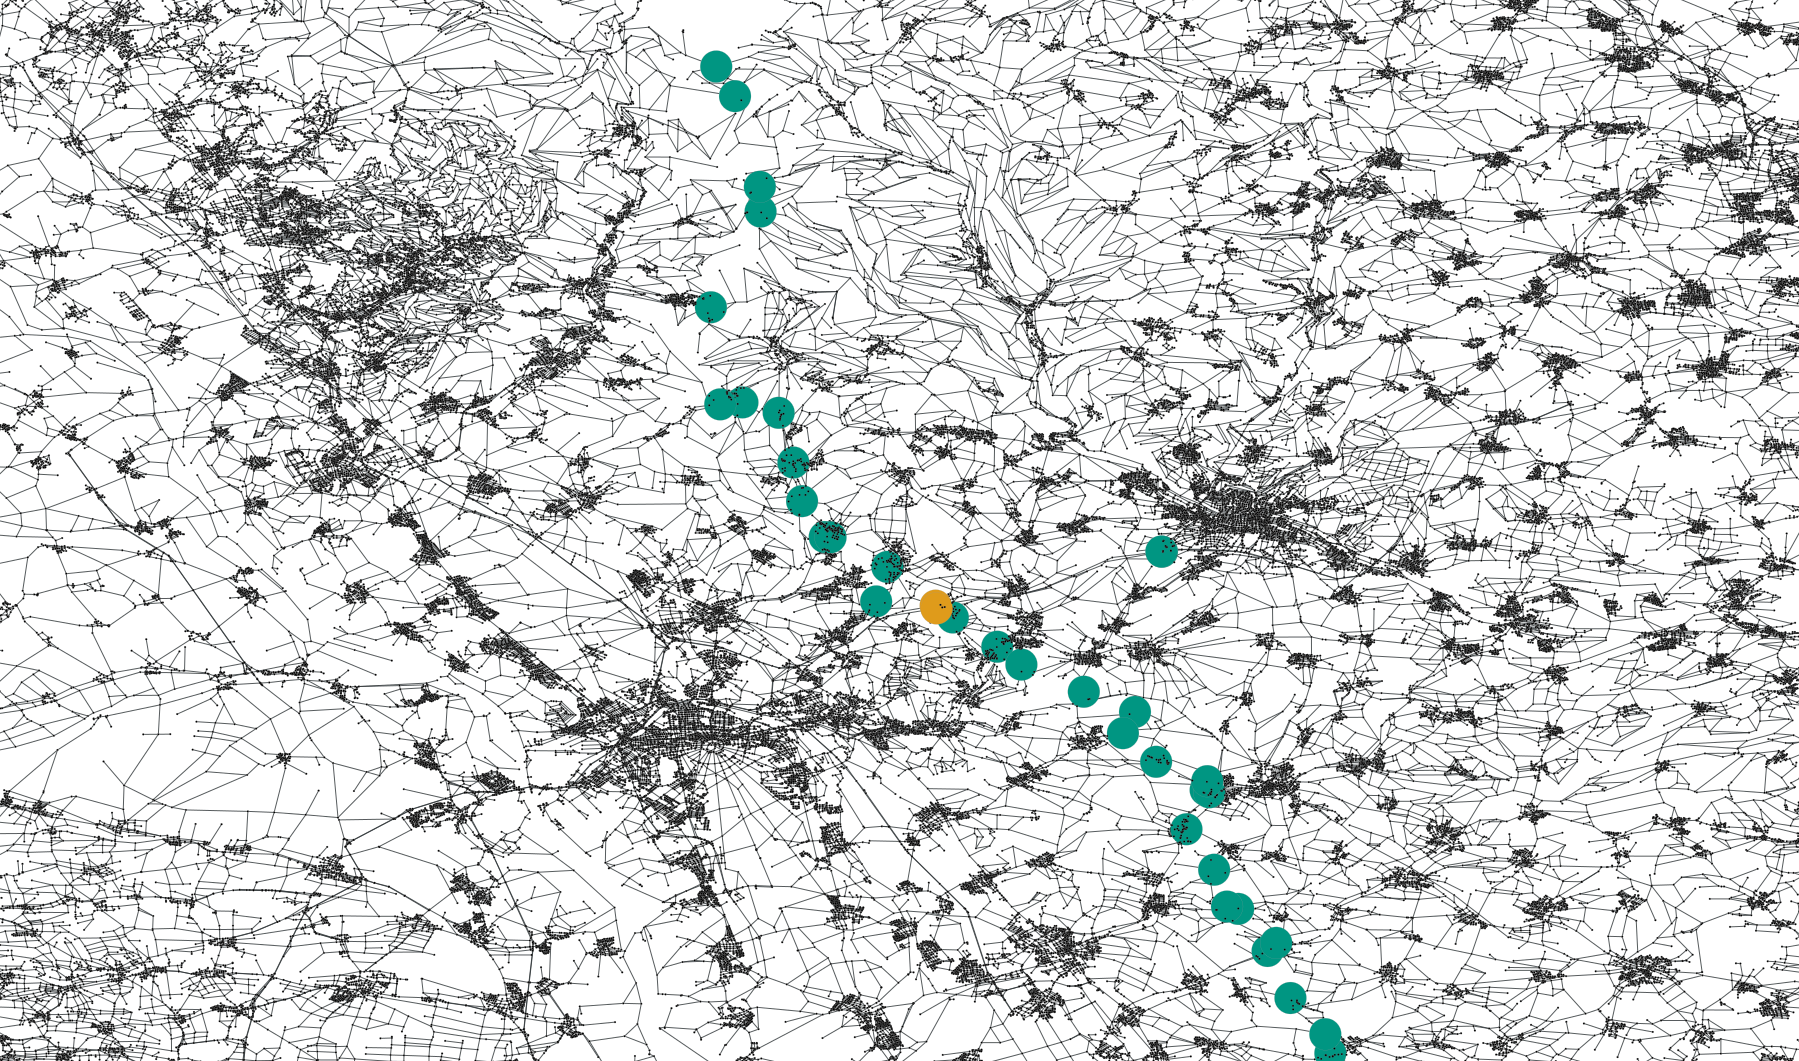
\includegraphics[width=0.7\linewidth]{graphics/karlsruhe_top_level_sep_extended_to_planar_wide.png}
    \caption{Visualization of a top-level separator for the road network of Karlsruhe. Vertices colored teal represent the separator nodes identified within the original, non-planar graph. Orange vertices indicate the additional nodes required to establish a valid separator for the planarized version of the network. The single teal vertex on the right is a highway intersection whose inclusion is necessary for the separator.}
    \label{fig:karlsruhe_planar_vs_non_planar}
\end{figure}

\begin{figure}[tbhp]
    \centering
    \begin{subfigure}{0.45\linewidth}
        \centering
        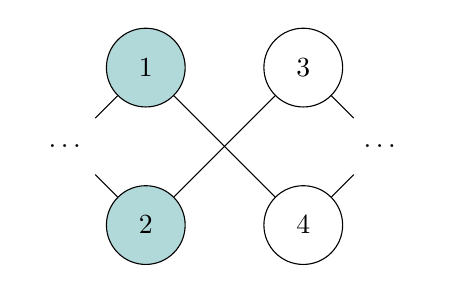
\begin{tikzpicture}[every node/.style={circle, draw, minimum size=1cm}]
            \node[draw=none] (dots1) at (0, 1) {\dots};
            \node[fill=teal!30] (1) at (1, 2) {1};
            \node[fill=teal!30] (2) at (1, 0) {2};
            \node (3) at (3, 2) {3};
            \node (4) at (3, 0) {4};
            \node[draw=none] (dots2) at (4, 1) {\dots};

            \draw (1) -- (4);
            \draw (2) -- (3);

            \draw (1) -- (dots1);
            \draw (2) -- (dots1);
            \draw (3) -- (dots2);
            \draw (4) -- (dots2);
        \end{tikzpicture}
        \caption{Separator in non-planar graph.}
    \end{subfigure}
    \hfill
    \begin{subfigure}{0.45\linewidth}
        \centering
        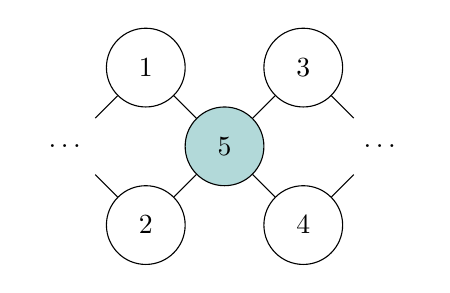
\begin{tikzpicture}[every node/.style={circle, draw, minimum size=1cm}]
            \node[draw=none] (dots1) at (0, 1) {\dots};
            \node (1) at (1, 2) {1};
            \node (2) at (1, 0) {2};
            \node (3) at (3, 2) {3};
            \node (4) at (3, 0) {4};
            \node[fill=teal!30] (5) at (2, 1) {5};
            \node[draw=none] (dots2) at (4, 1) {\dots};

            \draw (1) -- (5);
            \draw (2) -- (5);
            \draw (3) -- (5);
            \draw (4) -- (5);

            \draw (1) -- (dots1);
            \draw (2) -- (dots1);
            \draw (3) -- (dots2);
            \draw (4) -- (dots2);
        \end{tikzpicture}
        \caption{Separator in planarized graph.}
    \end{subfigure}
    \caption{Example of a separator that decreases in size after planarization.}
    \label{fig:planarization_reduces_separator}
\end{figure}

\begin{figure}[tbhp]
    \centering
    \begin{subfigure}{0.45\linewidth}
        \centering
        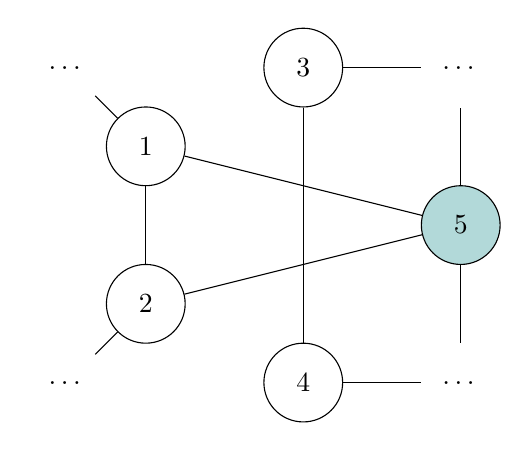
\begin{tikzpicture}[every node/.style={circle, draw, minimum size=1cm, node distance=1.5cm}]
            \node[draw=none] (ldots1) at (0,0) {\dots};
            \node[draw=none] (ldots2) at (0,4) {\dots};
            \node (1) at (1,3) {1};
            \node (2) at (1,1) {2};
            \node (3) at (3,4) {3};
            \node (4) at (3,0) {4};
            \node[fill=teal!30] (5) at (5,2) {5};
            \node[draw=none] (rdots1) at (5,0) {\dots};
            \node[draw=none] (rdots2) at (5,4) {\dots};

            \draw (ldots1) -- (2);
            \draw (ldots2) -- (1);
            \draw (1) -- (2);
            \draw (1) -- (5);
            \draw (2) -- (5);
            \draw (3) -- (4);
            \draw (3) -- (rdots2);
            \draw (4) -- (rdots1);
            \draw (5) -- (rdots1);
            \draw (5) -- (rdots2);
        \end{tikzpicture}
        \caption{Separator in non-planar graph.}
    \end{subfigure}
    \hfill
    \begin{subfigure}{0.45\linewidth}
        \centering
        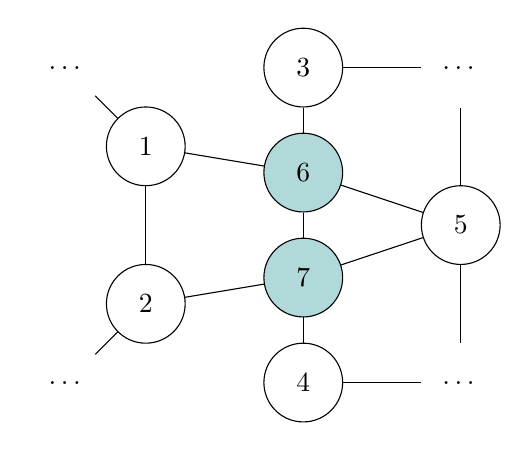
\begin{tikzpicture}[every node/.style={circle, draw, minimum size=1cm, node distance=1.5cm}]
            \node[draw=none] (ldots1) at (0,0) {\dots};
            \node[draw=none] (ldots2) at (0,4) {\dots};
            \node (1) at (1,3) {1};
            \node (2) at (1,1) {2};
            \node (3) at (3,4) {3};
            \node (4) at (3,0) {4};
            \node (5) at (5,2) {5};
            \node[draw=none] (rdots1) at (5,0) {\dots};
            \node[draw=none] (rdots2) at (5,4) {\dots};
            \node[fill=teal!30] (6) at (3, 2.6666) {6};
            \node[fill=teal!30] (7) at (3, 1.3333) {7};

            \draw (ldots1) -- (2);
            \draw (ldots2) -- (1);
            \draw (1) -- (2);
            \draw (3) -- (rdots2);
            \draw (4) -- (rdots1);
            \draw (5) -- (rdots1);
            \draw (5) -- (rdots2);
            \draw (3) -- (6) -- (7) -- (4);
            \draw (1) -- (6) -- (5);
            \draw (2) -- (7) -- (5);
        \end{tikzpicture}
        \caption{Separator in planarized graph.}
    \end{subfigure}
    \caption{Example of a separator that increases in size after planarization.}
    \label{fig:planarization_increases_separator}
\end{figure}


These findings highlight that the near-planar structure of road networks has minimal impact on separator size, suggesting that such networks can typically be analyzed as planar graphs without losing essential separator properties.

\section{Hierarchy}
\label{sec:hierarchy}

Real-world road networks possess a hierarchical structure.
Different types of roads cater to different travel distances and volumes, forming levels within the network.
Depending on the specific taxonomy used, road networks are categorized into various numbers of classes or levels.
For instance, a common classification for Germany includes:

\begin{itemize}
    \item Federal Motorways (Bundesautobahnen)
    \item Federal Highways (Bundesstraßen)
    \item State Roads (Landesstraßen)
    \item District Roads (Kreisstraßen)
    \item Municipal Roads (Gemeindestraßen)
\end{itemize}

\section{Diameter and Distance Distributions}
\label{sec:diameter}

The diameter of a graph, defined as the longest shortest path between any pair of vertices, is a fundamental metric characterizing its overall extent and the efficiency of traversal.
In our analysis, we focus specifically on the hop diameter, where each edge has a uniform weight of 1.
This choice is motivated by the desire to understand the graph's topological and hierarchical structure.
To ensure that the measured hop distances are structurally meaningful, we first pre-process all graphs and subgraphs by contracting vertices of degree 2.
This effectively treats long chains of such vertices as single conceptual edges.

Computing the exact diameter of a general graph can be computationally intensive.
A simple two-step Breadth-First Search (BFS) approach can be used. This involves performing a BFS from a random node to find the furthest vertex, and then a second BFS from that resulting vertex. However, this method is only guaranteed to find the exact diameter in certain graph classes, such as trees, and provides at best a 2-approximation for general graphs.
Therefore, to obtain exact diameter values, we employ the more sophisticated iFUB (iterative Fringe Upper Bound) algorithm as described by Crescenzi et al. \cite{crescenzi_computing_2013}.
This algorithm successfully computes the exact graph diameter in reasonable time on road networks without resorting to a full all-pairs shortest path calculation.

We investigate how the hop diameter scales with graph size by analyzing subgraphs obtained from the nested dissection process.
Our empirical analysis of these contracted subgraphs indicates that their diameter scales approximately as \bigO{n^{1/3}}.
This observed scaling behavior is illustrated in \cref{fig:road_network_diameter_scaling}.

\begin{figure}[tbhp]
    \centering
    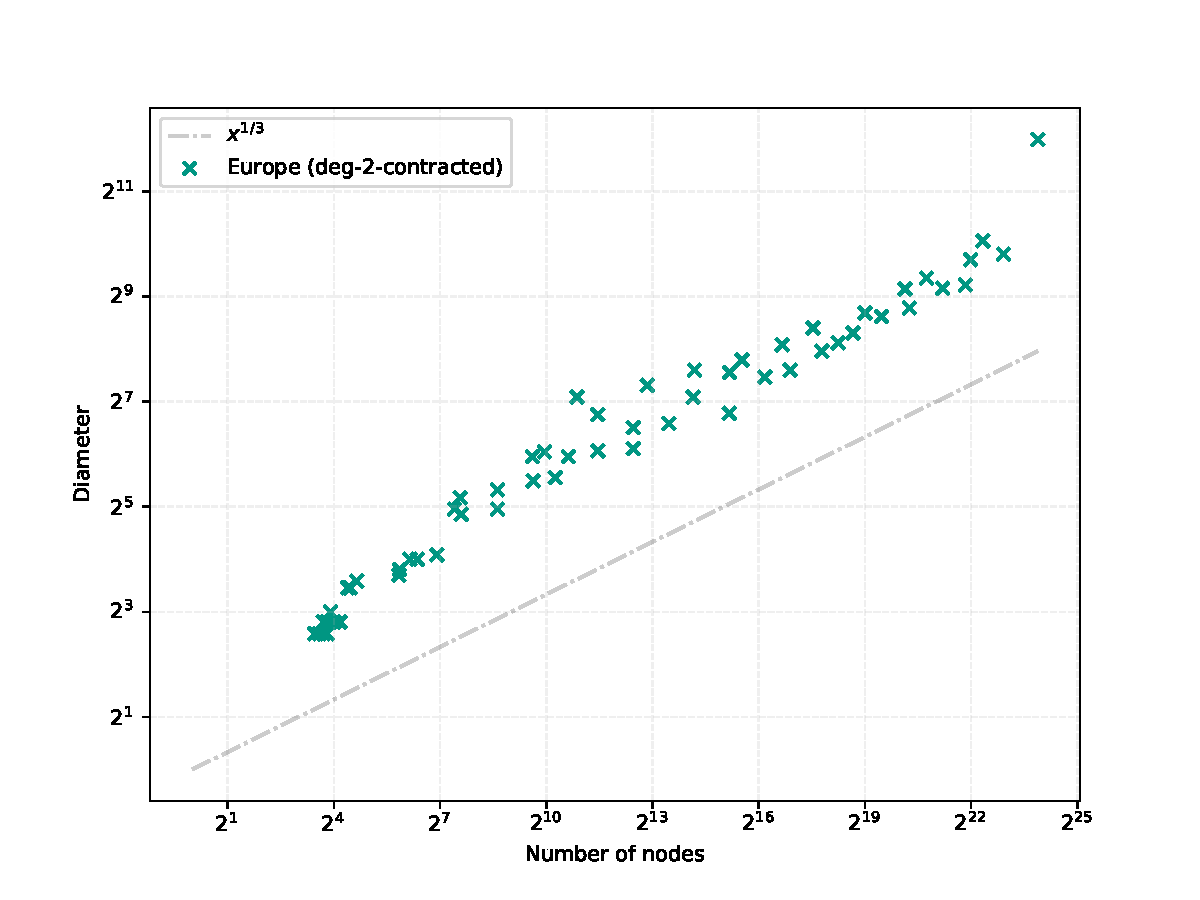
\includegraphics[width=0.6\linewidth]{graphics/diam-europe-ifub.pdf}
    \caption{Empirical scaling of hop diameter with the number of vertices \(n\) for nested dissection subgraphs of road networks (with degree-2 nodes contracted). The observed scaling is approximately \bigO{n^{1/3}}.}
    \label{fig:road_network_diameter_scaling}
\end{figure}

Beyond the maximum path length (diameter), we also analyze the complete distributions of both weighted distances and hop counts to understand typical path lengths.
Computing all-pairs shortest paths is computationally prohibitive for large graphs.
Therefore, we approximate these distributions by sampling \(10^4\) source nodes and performing a one-to-all shortest path query from each.
For the hop distance calculation, the graph is pre-processed by contracting all degree-2 vertices, consistent with our diameter analysis.
\cref{fig:distance_hop_distribution} visualizes the resulting frequencies for both metrics.

The two histograms reveal a key distinction between the network's geographic and topological structure.
The weighted distance distribution is strongly right-skewed with a smoothly decaying tail.
In contrast, the hop count distribution exhibits a sharp peak at a low hop count and has a significantly heavier tail.
We hypothesize that this heavy tail in the hop distribution is not an intrinsic topological property of the road network's hierarchy, but rather an artifact of the non-convex, geographically elongated shape of the European continent.
Even with a highly efficient network, paths between extremities, such as from Finland to Spain, are inherently long in terms of the number of intermediate junctions and segments.
This hypothesis is supported by two key observations.
First, the hop distribution for the more compact and convex graph of Germany does not exhibit a similarly heavy tail.
Second, we performed an experiment where points were sampled uniformly at random within the geographic shape of Europe, and a edge length restricted Delaunay triangulation was constructed on these points.
The hop distribution of this simple geometric graph also displays a very similar heavy tail.
This strongly suggests that the observed heavy tail in the Europe road network's hop distribution is primarily a consequence of its large-scale geography, rather than a feature of its specific man-made topology.


\begin{figure}[tbhp]
    \centering
    \begin{subfigure}{0.45\linewidth}
        \centering
        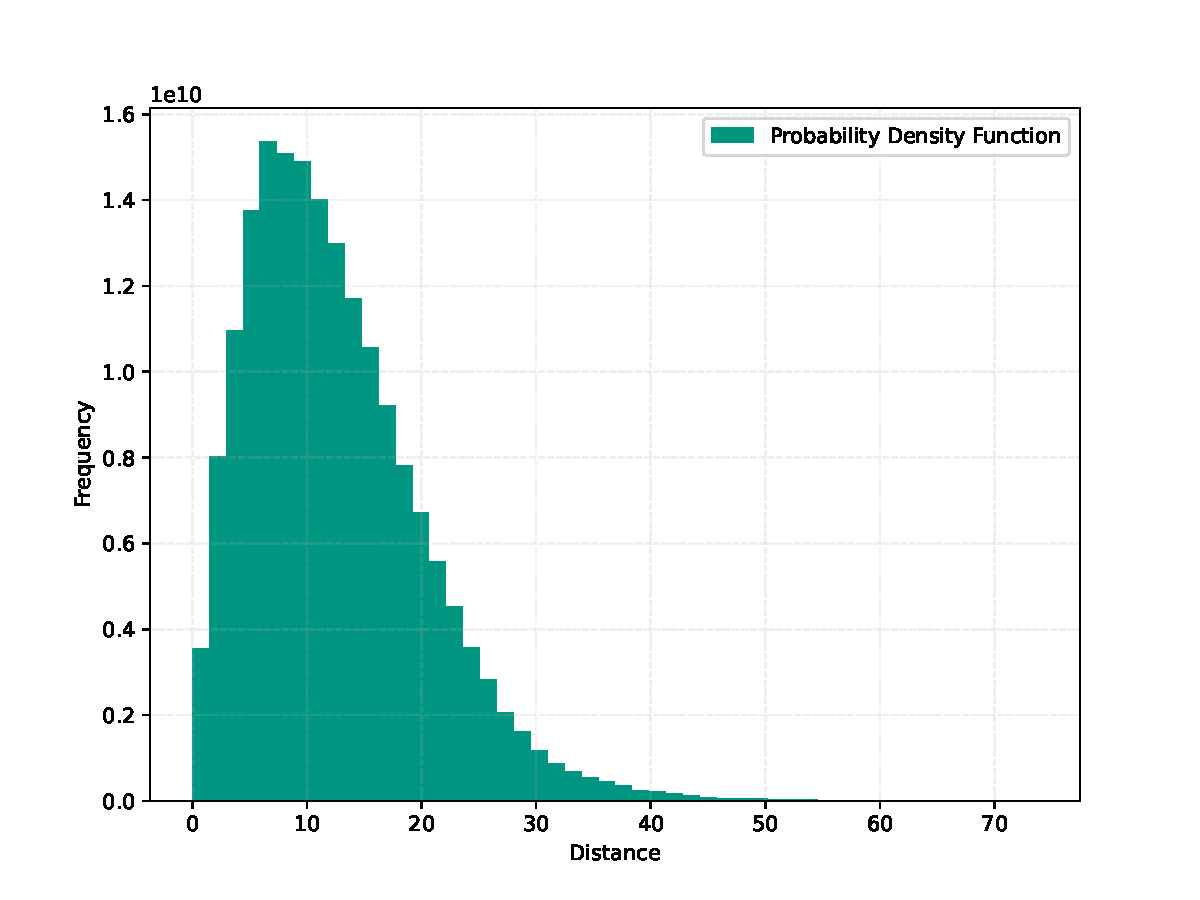
\includegraphics[width=\linewidth]{graphics/distances_europe.pdf}
        \caption{Distribution of weighted path distances for the Europe network.}
        \label{fig:distance_distribution}
    \end{subfigure}
    \hfill
    \begin{subfigure}{0.45\linewidth}
        \centering
        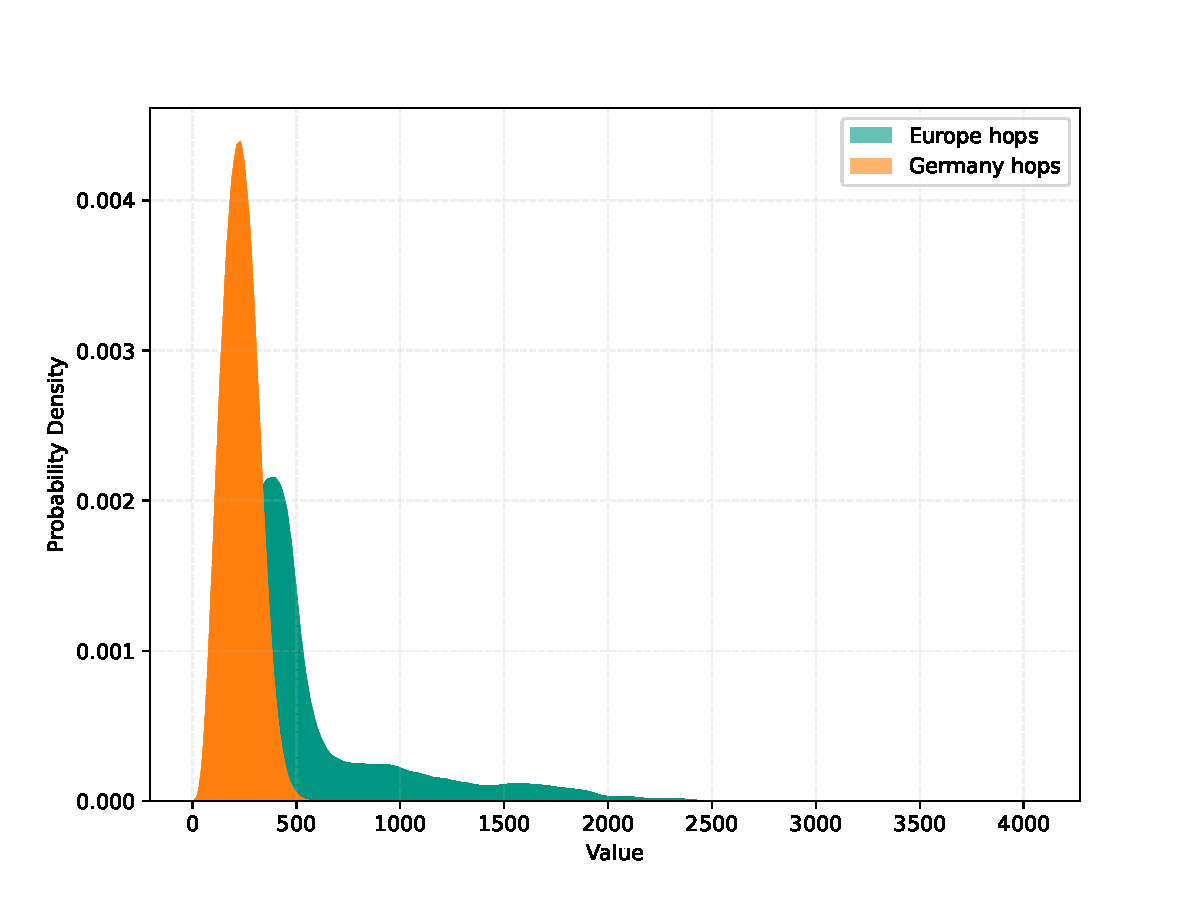
\includegraphics[width=\linewidth]{graphics/hops_europe_germany.pdf}
        \caption{Comparison of hop distance distributions for the Europe and Germany networks.}
        \label{fig:hop_distribution}
    \end{subfigure}
    \caption{Path length distributions approximated from 10,000 one-to-all queries. Left: Weighted distances for the DIMACS Europe road network. Right: Comparison of hop distributions for the Europe network versus the more compact Germany sub-network.}
    \label{fig:distance_hop_distribution}
\end{figure}
